\documentclass[12pt, oneside]{article}

\usepackage[letterpaper, scale=0.8, centering]{geometry}
\usepackage{fancyhdr}
\setlength{\parindent}{0em}
\setlength{\parskip}{1em}

\pagestyle{fancy}
\fancyhf{}
\renewcommand{\headrulewidth}{0pt}
\rfoot{{\footnotesize Copyright Mia Minnes, 2024, Version \today~(\thepage)}}

\usepackage{titlesec}

\author{CSE20S24}

\newcommand{\instructions}{{\bf For all HW assignments:} 
These homework assignments may be done individually or in groups of up to 3 students.
Please ensure your name(s) and PID(s)
are clearly visible on the first page of your homework
submission, start each question on a new page, and upload the PDF to Gradescope.
If you're working in a group, {\it submit only one submission per group}: one partner uploads the
submission through their Gradescope account and then adds the other group member(s) to the Gradescope submission
by selecting their name(s) in the ``Add Group Members'' dialog box. You will need to re-add your group member(s)
every time you resubmit a new version of your assignment.

Each homework question will be graded either for
{\bf correctness} (including clear and precise explanations and justifications of all answers) or
{\bf fair effort completeness}. You may collaborate on ``graded for correctness''
questions only with CSE 20 students in your group; if your
 group has questions about a problem, you may ask in drop-in help hours or post a private
post (visible only to the Instructors) on Piazza.  
 For ``graded for completeness''
 questions: collaboration is allowed with any CSE 20 students this quarter; 
 if your group has questions about a problem, you may ask in drop-in 
 help hours or post a public post on Piazza.

All submitted homework for this class must be typed. 
You can use a word processing editor if you like (Microsoft Word, Open Office, Notepad, Vim, Google Docs, etc.) 
but you might find it useful to take this opportunity to learn LaTeX. 
LaTeX is a markup language used widely in computer science and mathematics. 
The homework assignments are typed using LaTeX and you can use the source files 
as templates for typesetting your solutions.

{\bf Integrity reminders}
\begin{itemize}
\item Problems should be solved together, not divided up between the partners. The homework is
designed to give you practice with the main concepts and techniques of the course, 
while getting to know and learn from your classmates.
\item You may not collaborate on homework questions graded for correctness with anyone other than your group members.
You may ask questions about the homework in office hours (of the instructor, TAs, and/or tutors) and 
on Piazza (as private notes viewable only to the Instructors).  
You \emph{cannot} use any online resources about the course content other than the class material 
from this quarter -- this is primarily to ensure that we all use consistent notation and
definitions (aligned with the textbook) and also to protect the learning experience you will have when
the `aha' moments of solving the problem authentically happen.
\item Do not share written solutions or partial solutions for homework with 
other students in the class who are not in your group. Doing so would dilute their learning 
experience and detract from their success in the class.
\end{itemize}

}

\newcommand{\gradeCorrect}{({\it Graded for correctness}) }
\newcommand{\gradeCorrectFirst}{\gradeCorrect\footnote{This means your solution 
will be evaluated not only on the correctness of your answers, but on your ability
to present your ideas clearly and logically. You should explain how you 
arrived at your conclusions, using
mathematically sound reasoning. Whether you use formal proof techniques or 
write a more informal argument
for why something is true, your answers should always be well-supported. 
Your goal should be to convince the
reader that your results and methods are sound.} }
\newcommand{\gradeComplete}{({\it Graded for completeness}) }
\newcommand{\gradeCompleteFirst}{\gradeComplete\footnote{This means you will 
get full credit so long as your submission demonstrates honest effort to 
answer the question. You will not be penalized for incorrect answers. 
To demonstrate your honest effort in answering the question, we 
expect you to include your attempt to answer *each* part of the question. 
If you get stuck with your attempt, you can still demonstrate 
your effort by explaining where you got stuck and what 
you did to try to get unstuck.} }

%\usepackage{tikz}
%\usetikzlibrary{circuits.logic.US,circuits.logic.IEC}

\usepackage{amssymb,amsmath,pifont,amsfonts,comment,enumerate,enumitem}
\usepackage{currfile,xstring,hyperref,tabularx,graphicx,wasysym}
\usepackage[labelformat=empty]{caption}
\usepackage{xcolor}
\usepackage{multicol,multirow,array,listings,tabularx,lastpage,textcomp,booktabs}

% NOTE(joe): This environment is credit @pnpo (https://tex.stackexchange.com/a/218450)
\lstnewenvironment{algorithm}[1][] %defines the algorithm listing environment
{   
    \lstset{ %this is the stype
        mathescape=true,
        frame=tB,
        numbers=left, 
        numberstyle=\tiny,
        basicstyle=\rmfamily\scriptsize, 
        keywordstyle=\color{black}\bfseries,
        keywords={,procedure, div, for, to, input, output, return, datatype, function, in, if, else, foreach, while, begin, end, }
        numbers=left,
        xleftmargin=.04\textwidth,
        #1
    }
}
{}
\lstnewenvironment{java}[1][]
{   
    \lstset{
        language=java,
        mathescape=true,
        frame=tB,
        numbers=left, 
        numberstyle=\tiny,
        basicstyle=\ttfamily\scriptsize, 
        keywordstyle=\color{black}\bfseries,
        keywords={, int, double, for, return, if, else, while, }
        numbers=left,
        xleftmargin=.04\textwidth,
        #1
    }
}
{}

\newcommand\abs[1]{\lvert~#1~\rvert}
\newcommand{\st}{\mid}

\newcommand{\A}[0]{\texttt{A}}
\newcommand{\C}[0]{\texttt{C}}
\newcommand{\G}[0]{\texttt{G}}
\newcommand{\U}[0]{\texttt{U}}

\newcommand{\cmark}{\ding{51}}
\newcommand{\xmark}{\ding{55}}





\title{hw4-proofs-and-sets}
\date{Due: 5/14/24 at 5pm (no penalty late submission until 8am next morning)}
\begin{document}
\maketitle
\thispagestyle{fancy}


{\bf In this assignment}, you will use propositional and predicate logic to evaluate
statements and arguments. You will analyze statements and determine if they are true or false using valid proof strategies.
You will also determine if candidate arguments are valid.


{\bf Relevant class material}: Weeks 4,5,6.

You will submit this assignment via Gradescope
(\href{https://www.gradescope.com}{https://www.gradescope.com}) 
in the assignment called ``hw4-proofs-and-sets''.

\instructions


\vspace{-10pt}

In your proofs and disproofs of statements below, justify each  step
by reference to  a component of the  following proof  strategies
we  have discussed so far, and/or to relevant definitions and calculations.

\vspace{-10pt}

\begin{itemize}
    \item A counterexample can be used to prove that  $\forall x P(x)$ is {\bf false}.
    \item  A witness can be used  to  prove that  $\exists x P(x)$ is {\bf true}.
    \item {\bf Proof of universal by exhaustion}: To prove that $\forall x \, P(x)$
is true when $P$ has a finite domain, evaluate the predicate at {\bf each} domain element to confirm that it is always T.
    \item  {\bf Proof by universal generalization}: To prove that $\forall x \, P(x)$
is true, we can take an arbitrary element $e$ from the domain and show that $P(e)$ is true, without making any assumptions about $e$ other than that it comes from the domain.
    \item To  prove  that $\exists x P(x)$ is {\bf false}, write the universal statement that is logically equivalent to its negation and then prove it true using universal generalization.
    \item {\bf Strategies for conjunction}: To prove that $p \land q$ is true, have two subgoals: subgoal (1) prove $p$ 
is  true; and, subgoal (2) prove $q$ is true. To prove that $p \land q$ is false, it's enough to prove that $p$ is false.
 To prove that $p \land q$ is false, it's enough to prove that $q$ is false.
    \item {\bf Proof of Conditional by Direct Proof}: To prove that the implication $p \to q$ is true, we can assume $p$ is true and use that assumption to show $q$ is true.
    \item {\bf Proof of Conditional by Contrapositive Proof}: To prove that the implication $p \to q$ is true, we can assume $\neg q$ is true and use that assumption to show $\neg p$ is true.
    \item {\bf Proof by Cases}: To prove $q$ when we know $p_1 \lor p_2$, show that $p_1 \to q$ and $p_2 \to q$.
\end{itemize}


{\bf Assigned questions}

\begin{enumerate}[labelindent=0pt, leftmargin=0pt]
    \item  Evaluating predicates. Consider the following predicates, each of which has 
    as its domain the set of all bitstrings whose leftmost bit is $1$
    
    $E(x)$ is $T$ exactly when $(x)_{2}$ is even, and is $F$ otherwise
    
    $L(x)$ is $T$ exactly when $(x)_2 < 15$, and is $F$ otherwise
    
    $M(x)$ is $T$ exactly when $(x)_2 > 2$ and is $F$ otherwise.
    
    
    \rule{0.5\textwidth}{.4pt}
    
    {\it Sample response that can be used as reference for the detail expected 
    in your answer:} To prove that the statement $$\forall x ~L(x)$$ is false, we can use 
    the counterexample $x = 1111$, which is a bitstring whose leftmost bit is $1$ (so is in the domain).
    Applying the definition of $L(x)$, since $(1111)_2 = 1 \cdot 2^3 + 1\cdot 2^2 + 1 \cdot 2^1 + 1 \cdot 2^0 = 8 + 4+2+1 = 15$
    which is not (strictly) less than $15$, we have that $L(1111) = F$ and so the universal statement is false.
    
    
    \rule{0.5\textwidth}{.4pt}
    
    
    
    \begin{enumerate}
    \item\gradeCorrectFirst Use a counterexample to prove that the statement
    \[
    \forall x ( ~L(x) \to E(x)~)
    \]
    is false.
    
    \item\gradeCorrect Use a witness to prove that the statement
    \[
    \exists x (~L(x) \land M(x) ~)
    \]
    is true.
    
    \item\gradeCompleteFirst Translate each of the statements in the previous two
    parts to English.
    \end{enumerate}


    \item Set properties. Let $W = \mathcal{P}(\{1,2,3,4,5\})$. 


    \rule{0.5\textwidth}{.4pt}
    
    {\it Sample response that can be used as reference for the detail expected 
    in your answer for parts (a) and (b) below:} 
    
    To give an example element in the set 
    $\{ X \in W ~|~ 1 \in X \} \cap \{ X \in W ~|~  2 \in X \}$,
    consider $\{ 1,2\}$. To prove that this is in the set, by definition of intersection, we need to show
    that $\{1,2\} \in \{ X \in W ~|~ 1 \in X \}$ and that $\{1,2\} \in \{ X \in W ~|~ 2 \in X \}$.
    \begin{itemize}
    \item By set builder notation, elements in $\{ X \in W ~|~ 1 \in X \}$ have to be elements of $W$ which have $1$ as an element. By definition of power set, elements of $W$ are subsets of $\{1,2,3,4,5\}$. Since
    each element in $\{1,2\}$ is an element of $\{1,2,3,4,5\}$, $\{1,2\}$ is a subset of $\{1,2,3,4,5\}$ 
    and hence is an element of $W$. Also, by roster method, $1 \in \{1,2\}$. Thus, $\{1,2\}$ satisfies the 
    conditions for membership in $\{ X \in W ~|~ 1 \in X \}$.
    \item Similarly, by set builder notation, elements in $\{ X \in W ~|~ 2 \in X \}$ have to be elements of $W$ 
    which have $2$ as an element. 
    By definition of power set, elements of $W$ are subsets of $\{1,2,3,4,5\}$. Since
    each element in $\{1,2\}$ is an element of $\{1,2,3,4,5\}$, $\{1,2\}$ is a subset of $\{1,2,3,4,5\}$ 
    and hence is an element of $W$. Also, by roster method, $2 \in \{1,2\}$. Thus, $\{1,2\}$ satisfies the 
    conditions for membership in $\{ X \in W ~|~ 2 \in X \}$.
    \end{itemize}
    
    \rule{0.5\textwidth}{.4pt}
    
    
    \begin{enumerate}
    \item\gradeCorrect Give two (different) example elements in 
    \[
    W \times \mathcal{P}(W)
    \]
    Justify your examples by explanations that include references to the relevant definitions.
    
    \item\gradeCorrect Give one example element in 
    \[
    \{ X \in W \mid (1 \in X) \land (X \cap \{3,4\} = \emptyset) \}
    \]
    Justify your example by explanations that include references to the relevant definitions.
    
    \item\gradeComplete Consider the following statement and attempted proof:
    
    
    $$\forall A \in W \, \forall B \in W ~\left(~((A \cap B) \subseteq A) \to (A \subseteq B)~\right)$$
    
    \begin{quote}
    (1) Towards a universal generalization argument, {\bf choose arbitrary} $A \in W, B \in W$ .
    
    (2) We need {\bf to show} $((A \cap B) \subseteq A) \to (A \subseteq B)$.
    
    (3) Towards a proof of the conditional by the contrapositive, {\bf assume} $A \subseteq B$, and we need {\bf to show} 
    that $(A \cap B) \subseteq A$.
    
    (4) By definition of subset inclusion, this means we need {\bf to show} 
    $\forall x ~( x \in A \cap B \to  x \in A  ~)$.
    
    (5) Towards a universal generalization, {\bf choose arbitrary} $x$; we need {\bf to show} that \\
    $x \in A \cap B \to x \in A$.
    
    (6) Towards a direct proof, {\bf assume} $x \in A \cap B$, and we need {\bf to show } $x \in A$.
    
    (7) By definition of set intersection and set builder notation, we have that $x \in A \land x \in B$.
    
    (8) By the definition of conjunction, $x \in A$, which is  what we needed to show. QED
    \end{quote}
    
    Demonstrate that this attempted proof is invalid by providing
    and justifying a {\bf counterexample} (disproving the statement).
    Then, explain why this attempted proof is 
    invalid by identifying in which step a definition or proof strategy is used incorrectly, and describing how the 
    definition or proof strategy was misused.

    \item \gradeComplete A Venn diagram is a chart of overlapping regions that illustrates the similarities
    differences of a collection of sets. You may have seen some examples in memes, including
    these (from a web search):
    \begin{center}
        \hfill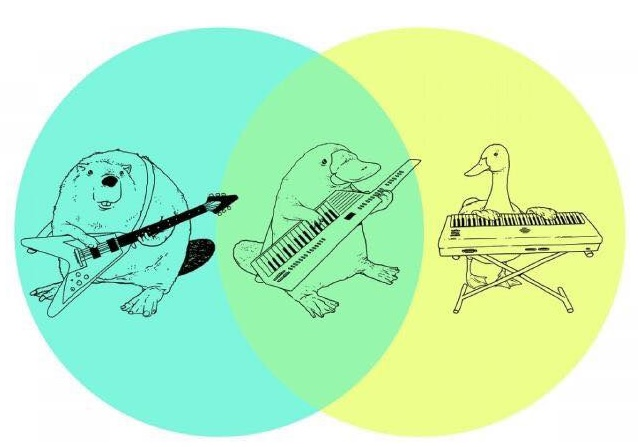
\includegraphics[width=1.5in]{../../resources/images/funny-pictures-venn-diagram-duck-5448120.jpeg} \hfill
        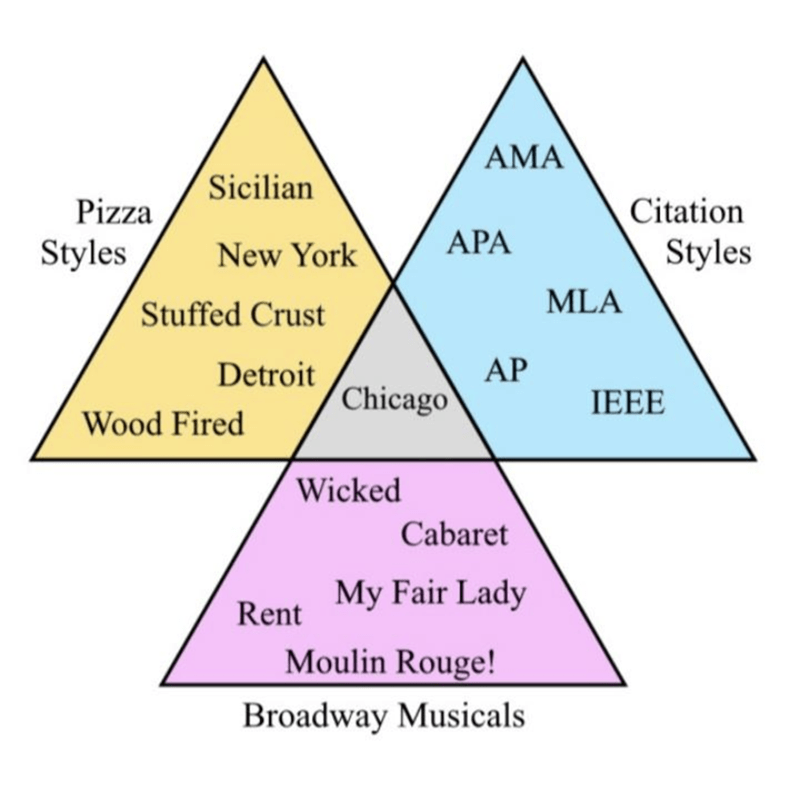
\includegraphics[width=1.5in]{../../resources/images/detroit-ap-chicago-ieee-wood-fired-wicked-cabaret-my-fair-lady-rent-moulin-rouge-broadway-musicals.png}
        \hfill
    \end{center}
    Mostly we see Venn Diagrams with 2 or 3 circles (or other shapes). In this question, 
    we consider how to draw a Venn Diagram with 4 regions.
    \begin{enumerate}
        \item Here is a Venn Diagram with 2 circles. Each region is labelled (encoded) with a 
        binary string with 2 bits. Notice that there are four regions: the region outside
        of the two circles, the region inside the left circle and not the right circle, the region 
        inside the right circle and not the left circle, and the region inside both circles.
        \begin{center}
            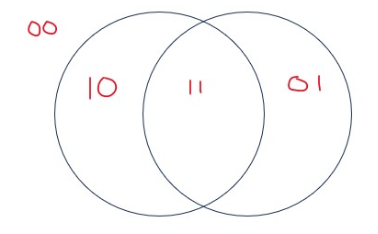
\includegraphics[width=1.5in]{../../resources/images/VennDiagram2Circles.png}
        \end{center}
        Generalize this encoding by encoding each region in this 3 circle Venn Diagram with 
        a unique binary string with 3 bits.
        \begin{center}
            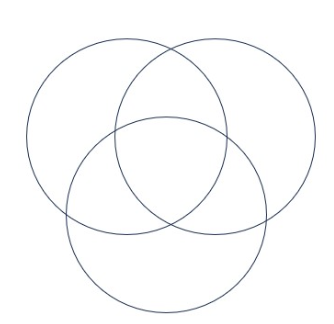
\includegraphics[width=1.5in]{../../resources/images/VennDiagram3Circles.png}
        \end{center}
        \item Give an alternate representation of the regions in the 2 circle and 3 circle 
        Venn Diagrams by labelling each circle with a letter ($X$, $Y$, $Z$, or $A$, $B$, $C$, for 
        example) and then expressing each region as the result of combining these with set operations
        (like union, intersection, and set difference).
        \item Here are two attempts at a Venn Diagram with 4 shapes, one with circles and the other 
        with ellipses.
        \begin{center}
            \hfill
            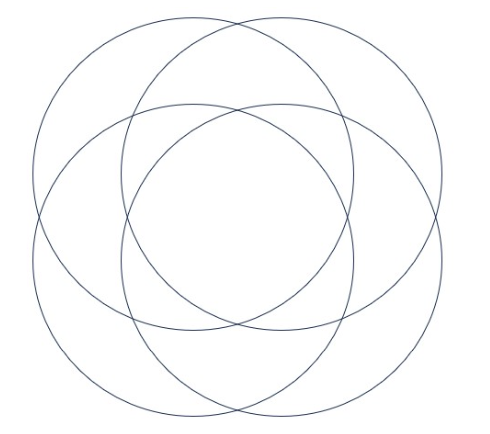
\includegraphics[width=1.5in]{../../resources/images/VennDiagram4Circles.png}
            \hfill 
            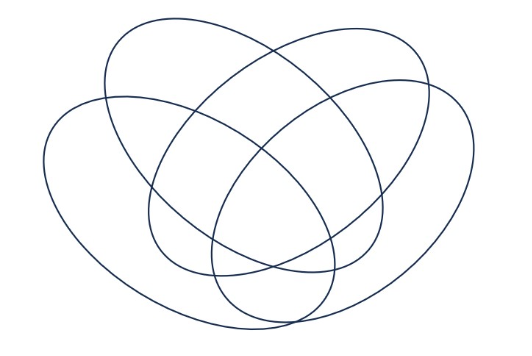
\includegraphics[width=1.5in]{../../resources/images/VennDiagram4Ellipses.png}
            \hfill
        \end{center}
        Is there anything missing from either diagram? (How many regions are there? 
        How many regions should there be in order to use each 4 bit binary string 
        exactly once in a generalization of the encoding we saw before?) 
        If you had to choose one of these diagrams, which would you choose, and why?
    \end{enumerate}
    (This question is adapted from one created by Miles Jones and is used with permission.)
    \end{enumerate}
    
    
    \item Number properties. Consider the predicate  $F(~(a,b)~)  = ``a \text{ is a factor of } b"$ 
    over  the domain $\mathbb{Z}^{\neq 0} \times \mathbb{Z}$. Consider the following quantified
    statements
    \begin{multicols}{2}
    \begin{enumerate}[label=(\roman*)]
    \item $\forall x \in \mathbb{Z} ~(F(~(1,x~)))$
    \item $\forall x \in \mathbb{Z}^{\neq 0} ~(F(~(x,1)~))$
    \item $\exists x \in \mathbb{Z} ~(F(~(1,x)~))$
    \item $\exists x \in \mathbb{Z}^{\neq 0} ~(F(~(x,1)~))$
    \item $\forall x \in \mathbb{Z}^{\neq 0} ~\exists y \in \mathbb{Z} ~(F(~(x,y)~))$
    \item $\exists x \in \mathbb{Z}^{\neq 0} ~\forall y \in \mathbb{Z} ~(F(~(x,y)~))$
    \item $\forall y \in \mathbb{Z} ~\exists x \in \mathbb{Z}^{\neq 0} ~(F(~(x,y)~))$
    \item $\exists y \in \mathbb{Z} ~\forall x \in \mathbb{Z}^{\neq 0} ~(F(~(x,y)~))$
    \end{enumerate}
    \end{multicols}
    
    \begin{enumerate}
    
    \item\gradeComplete
    Which of the statements (i) - (viii) is being {\bf proved} by the following proof:
    
    \begin{quote}
      By universal generalization, {\bf choose} $e$ to be an {\bf arbitrary} integer. 
      We need to show that $F(~(1,e)~)$. By definition of the  predicate $F$, we can rewrite 
      this goal as $\exists c \in \mathbb{Z}~(e = c \cdot 1)$. We pick the {\bf witness} $c = e$, 
      which is an integer and therefore in the domain. Calculating, 
      $c \cdot 1 = e \cdot 1 = e$, as required. Since the predicate $F(1,e)$ evaluates to true 
      for the arbitrary integer $e$, the claim has been proved. $\square$
    \end{quote}
    
    
    {\it Hint: it may be useful to 
    identify the key words in the proof that indicate proof strategies.}
    
    \item\gradeComplete
    Which of the statements (i) - (viii) is being {\bf disproved} by the following proof:
    
    \begin{quote}
      To disprove the statement, we need to find a counterexample. We choose $2$, a nonzero
      integer so in the domain. We need to show that $\lnot F(~(2,1)~)$. By definition of the predicate $F$, we 
      can rewrite this goal as $1 \textbf{ mod } 2 \neq 0$. By definition of integer division, since 
      $1 = 0 \cdot 2  + 1$ (and $0 \leq 1 < 2$), $1 \textbf { mod } 2 = 1$ which is nonzero so the counterexample works to 
      disprove the original statement.
       $\square$
    \end{quote}
    
    {\it Hint: it may be useful to 
    identify the key words in the proof that indicate proof strategies.}
    
    \item ({\it Graded for correctness of evaluation of statement (is it true or false?) and fair effort completeness of the translation and proof}) 
    Translate the statement to English, state whether is it true or false, and then justify your answer (by proving the statement or its negation).
    $$\exists x \in \mathbb{Z}^{\neq 0}~ \exists y \in \mathbb{Z}^{\neq 0} ~(~\lnot(x = y) \land F(~(x,y)~) \land F(~(y,x)~)~)$$
    
    \item ({\it Graded for correctness of evaluation of statement (is it true or false?) 
    and fair effort completeness of the translation and of the proof}) 
    Translate the statement to English, state whether is it true or false, and then justify your answer (by proving the statement or its negation).
    $$\forall x \in \mathbb{Z}^{\neq 0}~ \forall y \in \mathbb{Z}^{\neq 0} ~(~F(~(x,y)~) \to \lnot F(~(y,x)~)~)$$
    
    \item ({\it Graded for correctness of evaluation of statement (is it true or false?) 
    and fair effort completeness of the translation and of the proof}) 
    Translate the statement to English, state whether is it true or false, and then justify your answer (by proving the statement or its negation).
    $$\exists x \in \mathbb{Z}^{\neq 0}~ \exists y \in \mathbb{Z}~(~F(~(x,y)~) \land  F(~(x+1, y)~) \land F(~(x+2, y)~)~)$$
    
    \item ({\it Graded for correctness of evaluation of statement (is it true or false?) 
    and fair effort completeness of the translation and of the proof}) 
    Translate the statement to English, state whether is it true or false, and then justify your answer (by proving the statement or its negation).
    $$\forall x \in \mathbb{Z}^{\neq 0}~ (~F(~(x,x^2)~) \land F(~(x,x^3)~)~)$$
    
    \end{enumerate}
    
    \item Structural induction. Recall that we define the set of bases as $B  =  \{ \A, \C, \U, \G \}$.
The set of RNA strands $S$ is defined (recursively) by:
\[
\begin{array}{ll}
\textrm{Basis Step: } & \A \in S, \C \in S, \U \in S, \G \in S \\
\textrm{Recursive Step: } & \textrm{If } s \in S\textrm{ and }b \in B \textrm{, then }sb \in S
\end{array}
\]
where $sb$ is string concatenation. 
The function \textit{rnalen} that computes the length of RNA strands in $S$ is defined recursively by
$rnalen: S  \to \mathbb{Z}^+$


\begin{quote}
Basis step: If $b \in B$ then $rnalen(b)  = 1$

Recursive step: If $s \in S$ and $b \in B$, then $rnalen(sb)  = 1 + rnalen(s)$
\end{quote}

The function \textit{basecount} that computes the number of a given base 
$b$ appearing in a RNA strand $s$ is defined recursively:
    
\[
\begin{array}{llll}
& & \textit{basecount} : S \times B & \to \mathbb{N} \\
\textrm{Basis Step:} &  \textrm{If } b_1 \in B, b_2 \in B & \textit{basecount}(~(b_1, b_2)~) & =
        \begin{cases}
            1 & \textrm{when } b_1 = b_2 \\
            0 & \textrm{when } b_1 \neq b_2 \\
        \end{cases} \\
\textrm{Recursive Step:} & \textrm{If } s \in S, b_1 \in B, b_2 \in B &\textit{basecount}(~(s b_1, b_2)~) & =
        \begin{cases}
            1 + \textit{basecount}(~(s, b_2)~) & \textrm{when } b_1 = b_2 \\
            \textit{basecount}(~(s, b_2)~) & \textrm{when } b_1 \neq b_2 \\
        \end{cases}
\end{array}
\]
\begin{enumerate}
\item ({\it Graded for correctness of evaluation of statement (is it true or false?) and fair effort completeness of the translation and proof}) 
Translate the statement to English, state whether is it true or false, and then justify your answer (by proving the statement or its negation).
$$\forall b \in B ~\exists s \in S ~(~rnalen(s) = basecount(~(s,b)~)~)$$

\item ({\it Graded for correctness of evaluation of statement (is it true or false?) 
and fair effort completeness of the translation and of the proof}) 
Translate the statement to English, state whether is it true or false, and then justify your answer (by proving the statement or its negation).
$$\forall s \in S~ (rnalen(s) > basecount( ~(s,\A)~))$$

\item ({\it Graded for correctness of evaluation of statement (is it true or false?) 
and fair effort completeness of the translation and of the proof}) 
Translate the statement to English, state whether is it true or false, and then justify your answer (by proving the statement or its negation).
$$\forall s \in S~ \forall b \in B ~( basecount( ~(s,b)~) > 0)$$

\end{enumerate}

\end{enumerate}
\end{document}
